\documentclass[t]{beamer}
\usetheme[deutsch]{KIT}
\setbeamercovered{transparent}
\setbeamertemplate{navigation symbols}{}

\KITfoot{Tutoriumsmaterial von Alexander Kwiatkowski, Michael Vollmer und Matthias Holoch \hspace{2.5cm} Basierend auf den Folien von Simon Stroh und Moritz v. Looz}
\usepackage[utf8]{inputenc}
\usepackage{amsmath}
\usepackage{ifthen}
\usepackage{amssymb}
\usepackage{tikz}
\usepackage{ngerman}
\usepackage[normalem]{ulem}
\usetikzlibrary{automata}
\usenavigationsymbols


\title{Theoretische Grundlagen der Informatik}
\subtitle{Tutorium}
\author{Alexander Kwiatkowski, Michael Vollmer und Matthias Holoch}

\institute[IKS]{Institut für Kryptographie und Sicherheit}

\TitleImage[height=\titleimageht]{images/tmaschine.png}

\newcommand{\N}{\ensuremath{\mathbb{N}}}
\newcommand{\M}{\ensuremath{\mathcal{M}}}
\newcommand{\classP}{\ensuremath{\mathcal{P}}}
\newcommand{\classNP}{\ensuremath{\mathcal{NP}}}
\newcommand{\co}{\ensuremath{\mathsf{co\text{-}}}}
\newcommand{\pot}{\ensuremath{\mathcal{P}}}
\newcommand{\abs}[1]{\ensuremath{\left\vert #1 \right\vert}}
\newcommand{\menge}[2]{\ensuremath{\left\lbrace #1 \,\middle\vert\, #2 \right\rbrace}}
\newcommand{\ducttape}[1]{\vspace{#1}}
\newcommand{\neglit}[1]{\overline{#1\vphantom{x^a}}}
\newcommand{\recipe}{\raisebox{-.3cm}{
\includegraphics[scale=.15]{images/chefs-cap.png}}\hspace{0.2cm}}
\newcommand{\opt}[1]{\ensuremath{\text{OPT}(#1)}}
\newcommand{\A}[1]{\ensuremath{\mathcal{A}(#1)}}
\renewcommand{\O}[1]{\ensuremath{\mathcal{O}(#1)}}
\newcommand{\msout}[1]{\text{\sout{\ensuremath{#1}}}}

\newcommand{\invincible}{\setbeamercovered{invisible}} %  "Yesss! I am invincible!!" (Boris Grishenko)
\newcommand{\vincible}{\setbeamercovered{transparent}}
\renewcommand{\solution}[1]{\invincible \pause #1 \vincible}
\newcommand{\micropause}{\\[8pt]}

% \@ifundefined{tikzset}{}{\tikzset{initial text=}} % Text "start" bei Startknoten unterdrücken
\tikzstyle{every node}=[thick]
\tikzstyle{every line}=[thick]

\newcommand{\tutnr}[1]{
  \subtitle{Tutorium #1}
	\begin{frame}
		\maketitle
	\end{frame}
}

\newcommand{\uebnr}[1]{
  \subtitle{Anmerkungen zum #1. Übungsblatt}
	\begin{frame}
		\maketitle
	\end{frame}
}

\begin{document}

\newcommand{\start}[3]
{
  \draw (#1*2,#2*2) node{$#3$};
  \draw (#1*2,#2*2) circle(0.4cm);
  \draw [->] (#1*2-0.9,#2) -- (#1*2-0.4,#2);
}
\newcommand{\final}[3]
{
  \draw (#1*2,#2*2) node{$#3$};
  \draw (#1*2,#2*2) circle(0.4cm);
  \draw (#1*2,#2*2) circle(0.32cm);
}
\newcommand{\startfinal}[3]
{
  \draw (#1*2,#2*2) node{$#3$};
  \draw (#1*2,#2*2) circle(0.4cm);
  \draw (#1*2,#2*2) circle(0.32cm);
  \draw [->] (#1*2-0.9,#2) -- (#1*2-0.4,#2);
}
\newcommand{\state}[3]
{
  \draw (#1*2,#2*2) node{$#3$};
  \draw (#1*2,#2*2) circle(0.4cm);
}
\newcommand{\tol}[4]
{
  \draw (#1+#3,#2*2) node[above]{$#4$};
  \draw [->] (#1*2-0.4,#2*2) -- (#3*2+0.4,#2*2);
}
\newcommand{\tor}[4]
{
  \draw (#1+#3,#2*2) node[above]{$#4$};
  \draw [->] (#1*2+0.4,#2*2) -- (#3*2-0.4,#2*2);
}
\newcommand{\tot}[4]
{
  \draw (#1*2,#2+#3) node[right]{$#4$};
  \draw [->] (#1*2,#2*2+0.4) -- (#1*2,#3*2-0.4);
}
\newcommand{\tob}[4]
{
  \draw (#1*2,#2+#3) node[right]{$#4$};
  \draw [->] (#1*2,#2*2-0.4) -- (#1*2,#3*2+0.4);
}
\newcommand{\totl}[5]
{
  \draw (#1+#3,#2+#4) node[above right]{$#5$};
  \draw [->] (#1*2-0.283,#2*2+0.283) -- (#3*2+0.283,#4*2-0.283);
}
\newcommand{\totr}[5]
{
  \draw (#1+#3,#2+#4) node[above left]{$#5$};
  \draw [->] (#1*2+0.283,#2*2+0.283) -- (#3*2-0.283,#4*2-0.283);
}
\newcommand{\tobl}[5]
{
  \draw (#1+#3,#2+#4) node[below right]{$#5$};
  \draw [->] (#1*2-0.283,#2*2-0.283) -- (#3*2+0.283,#4*2+0.283);
}
\newcommand{\tobr}[5]
{
  \draw (#1+#3,#2+#4) node[below left]{$#5$};
  \draw [->] (#1*2+0.283,#2*2-0.283) -- (#3*2-0.283,#4*2+0.283);
}
\newcommand{\rloopl}[3]
{
  \draw (#1*2-1,#2*2) node[left]{$#3$};
  \draw [->] (#1*2-0.35,#2*2-0.2) arc (-30:-320:0.32cm);
}
\newcommand{\rloopr}[3]
{
  \draw (#1*2+1,#2*2) node[right]{$#3$};
  \draw [->] (#1*2+0.35,#2*2+0.2) arc (150:-140:0.32cm);
}
\newcommand{\rloopt}[3]
{
  \draw (#1*2,#2*2+1) node[above]{$#3$};
  \draw [->] (#1*2-0.2,#2*2+0.35) arc (240:-50:0.32cm);
}
\newcommand{\rloopb}[3]
{
  \draw (#1*2,#2*2-1) node[below]{$#3$};
  \draw [->] (#1*2+0.2,#2*2-0.35) arc (60:-230:0.32cm);
}
\newcommand{\lloopl}[3]
{
  \draw (#1*2-1,#2*2) node[left]{$#3$};
  \draw [->] (#1*2-0.35,#2*2+0.2) arc (30:320:0.32cm);
}
\newcommand{\lloopr}[3]
{
  \draw (#1*2+1,#2*2) node[right]{$#3$};
  \draw [->] (#1*2+0.35,#2*2-0.2) arc (-150:140:0.32cm);
}
\newcommand{\lloopt}[3]
{
  \draw (#1*2,#2*2+1) node[above]{$#3$};
  \draw [->] (#1*2+0.2,#2*2+0.35) arc (-60:230:0.32cm);
}
\newcommand{\lloopb}[3]
{
  \draw (#1*2,#2*2-1) node[below]{$#3$};
  \draw [->] (#1*2-0.2,#2*2-0.35) arc (-240:50:0.32cm);
}
\include{amsmath}

\tutnr{12}

\section{Begriffe der Informationstheorie}
\subsection{Erklärung}
\begin{frame}
	\frametitle{Shannonscher Informationsbegriff}
	\begin{itemize}
		\item Jede Information bzw. Nachricht besitzt eine Quelle
		\begin{itemize}
			\item Oft randomisiert a.k.a. Zufallsquellen
			\item Wenn alle gesendete Nachrichten unabhängig voneinander sind, ist die Quelle gedächtnislos
		\end{itemize}
		\item Es gibt immer einen Empfänger, der die Nachrichten beobachtet
		\item Je unvorhersehbarer die Nachricht, desto mehr Informationsgehalt
		\begin{itemize}
				\item Wird deshalb auch manchmal Überraschungswert genannt
		\end{itemize}
		\item Entropie ist ein Begriff für die Dichte der Informationen
	\end{itemize}
\end{frame}

\begin{frame}
	\frametitle{Etwas genauer}
	\begin{itemize}
		\item Informationsgehalt soll nicht negativ sein
		\item Ein sicheres Ergebnis (p = 1) enthält keine Information
		\item Informationen von unabhängigen Nachrichten sollen sich addieren
		\item Kleine Änderungen der Wahrscheinlichkeit $\Rightarrow$ kleine Änderung des Informationsgehalts
		\item $I(x) = -log_b(p(x)) = log_b(\frac{1}{p(x)})$ erfüllt diese Bedingungen
		\begin{itemize}
			\item Meist wird als Basis b = 2 verwendet
		\end{itemize}~\\~\\
		\item Entropie ist entsprechend definiert~\\ $H(X) = \sum\limits_{x \in X} (p(x) \cdot log_2(\frac{1}{p(x)}) = \sum\limits_{x \in X} (p(x) \cdot I(x))$
	\end{itemize}
\end{frame}

\begin{frame}
	\frametitle{Beispiele}
	\begin{itemize}
		\item Zufallsquelle 1: p(A) = $\frac{1}{2}$, p(B) = $\frac{1}{2}$
		\item I(A) = $log_2(\frac{1}{0.5}) = log_2(2) = 1$ = I(B)
		\item H(X) = $(p(A) \cdot I(A)) + (p(B) \cdot I(B)) = 0.5 + 0.5 = 1$~\\~\\~\\~\\
		\item Zufallsquelle 2: p(A) = $\frac{1}{16}$, p(B) = $\frac{15}{16}$
		\item I(A) = $log_2(\frac{1}{0.0625}) = log_2(16) = 4$
		\item I(B) = $log_2(\frac{1}{0.9375}) = log_2(\frac{16}{15}) = 0.0931\ldots$
		\item H(X) = $(p(A) \cdot I(A)) + (p(B) \cdot I(B))$~\\$= (\frac{1}{16} \cdot 4) + (\frac{15}{16} \cdot 0.0931) = \frac{1}{4} + 0.873 = 0.337$
	\end{itemize}
\end{frame}
%Explaining "Ordnung von Zeichenketten would be Bogus"

\subsection{Aufgabe B11 A1}
\begin{frame}
	\frametitle{Aufgabe B11 A1}
	\begin{enumerate}
		\item Wie gro"s sind der Informationsgehalt und die Entropie, wenn eine Quelle mit
		dem Alphabet $\{0,1\}$ nur aus dem Zeichen $0$ bestehende Folgen sendet?
		\item An einer Quelle mit $n$ Zeichen tritt jedes Zeichen gleichverteilt auf. Wie
		gro"s sind der Informationsgehalt und die Entropie eines einzelnen Zeichens?
		\item Berechnen Sie die Entropie des Wurfes eines idealen W"urfels mit 8 Seiten,
		dessen Wahrscheinlichkeit f"ur jede Seite $p = \frac{1}{8}$ ist!
		\item Was ist der Unterschied zwischen den beiden Folgen, die aus verschiedenen
		ged"achtnislosen Quellen mit der gleichen Wahrscheinlichkeit f"ur $0$ und $1$
		gesendet werden, wenn man sie unter dem Aspekt Entropie und Ordnung betrachtet?
		\begin{enumerate}
			\item ...10101010101010101010...
			\item ...01101100110111000010...
		\end{enumerate}
	\end{enumerate}
\end{frame}

\section{Mehr Begriffe der Informationstheorie}
%Erklären: Empfänger, Kanäle, Verbundentropie, Äquivokation, Transinformation, Fehlinformation(="inverse Äquivokation"=Irrelevanz?), Totalinformation (=Verbundentropie?)
\begin{frame}
\frametitle{Übertragung von Information}
Daten können über einen Kanal von der Quelle zu einem Empfänger gesendet werden. Dieser Kanal ist in der Regel nicht störungsfrei, dass heißt die gesendeten Daten können ungleich zu den empfangenen sein.\\ 
Ein gestörter Kanal kann durch seine Übertragungswahrscheinlichkeiten $P(r|q)$, welche angeben wie wahrscheinlich es ist, dass r beim Empfänger ankommt, wenn q aus der Quelle gesendet wurde, charakterisiert werden.\\
Damit ergibt sich der Zusammenhang \[P(R=r)=\sum_{q \in Q} P(Q=q)P(R=r|Q=q)\] und für die Wahrscheinlichkeit das r und q gleichzeitig auftreten: \[P(Q=q,R=r)=P(Q=q)P(R=r|Q=q).\]
\end{frame}
\begin{frame}
\frametitle{Einige Definitionen}
\emph{Totalinformation} oder auch Verbundentropie H(Quelle $Q$, Empfänger $R$) ist die gesamte von Quelle und Empfänger erzeugte Entropie
\[H(Q,R)=-\sum_{q \in Q} \sum_{r \in R} P(Q=q,R=r)\log(P(Q=q,R=r))\]
\emph{Äquivokation} $H$(Quelle $Q|$ Empfänger $R$) gibt dem Entropieverlust durch die Übertragung an.\\
\[H(Q|R)=H(Q,R)-H(R)\]
\emph{Fehlinformation} H(Empfänger $R|$ Quelle $Q$) entspricht dem anscheinenden Entropiegewinn durch die Übertragung.
\[H(R|Q)=H(Q,R)-H(Q)\]
\emph{Transinformation} I(Quelle $Q$, Empfänger $R$) ist die richtig empfangene Informationsmenge.
\[I(Q,R)= H(Q)-H(Q|R)=H(R)-H(R|Q)=H(Q)+H(R)-H(Q,R)\]
\end{frame}
\begin{frame}
\frametitle{Bild zur Veranschaulichung}
\begin{center}
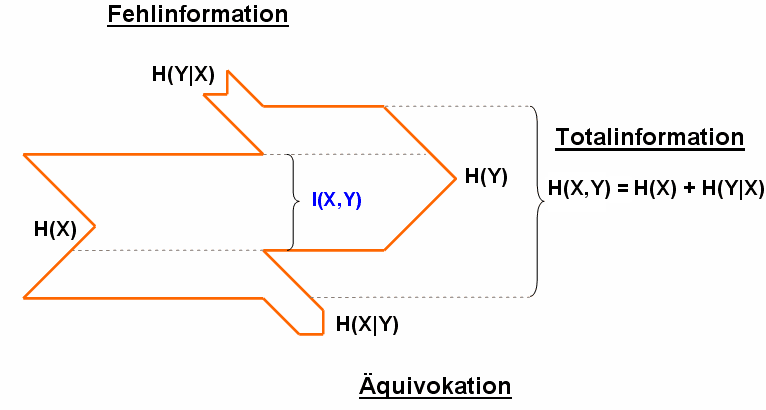
\includegraphics[scale=0.35]{images/Entropie_XY}
\end{center}
\end{frame}
\subsection{Erklärung}
\subsection{Aufgabe B11 A2}
\begin{frame}
	\frametitle{Aufgabe B11 A2}
	\only<1>{
	Studieren Sie den Fall eines asymmetrischen bin"aren Kanals mit Quelle $X$ und
	Empf"anger $Y$. Die "Ubertragungswahrscheinlichkeiten $P(Y|X)$ seien durch das
	folgende Diagramm gegeben:
	}
	\only<2->{
	\vspace{-0.6cm}
	}
		\begin{center}
			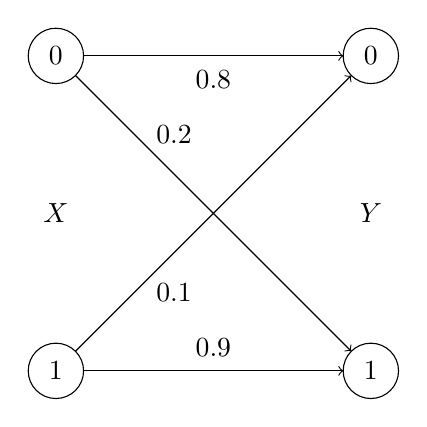
\begin{tikzpicture}
			\draw (0,0) circle (10pt);
			\draw (0,0) node {$1$};
			\draw (0,2) node {$X$};
			\draw (0,4) circle (10pt);
			\draw (0,4) node {$0$};
			\draw (4,0) circle (10pt);
			\draw (4,0) node {$1$};
			\draw (4,2) node {$Y$};
			\draw (4,4) circle (10pt);
			\draw (4,4) node {$0$};
			\draw [->] (0.35,0) -- (3.65,0);
			\draw (2,0.3) node {$0.9$};
			\draw [->] (0.35,4) -- (3.65,4);
			\draw (2,3.7) node {$0.8$};
			\draw [->] (0.25,0.25) -- (3.75,3.75);
			\draw (1.5,1) node {$0.1$};
			\draw [->] (0.25,3.75) -- (3.75,0.25);
			\draw (1.5,3) node {$0.2$};
			\end{tikzpicture}
		\end{center}
		\only<2,3>{
	\begin{enumerate}
		\only<2>{
		\item Wie gro"s ist die Wahrscheinlichkeit daf"ur, dass die Bitkette ``$1100$'' als
		``$1001$'' "ubertragen wird?
		\item Wenn die Entropie der Quelle $H(X) = 1 \; \mbox{bit}$ ist, wie gro"s ist dann
		$H(Y)$?
		\item Wie gro"s muss $H(X)$ sein, damit $H(Y) = 1 \; \mbox{bit}$ gilt?
		}
		\only<3>{
		\item Wie gro"s ist die Verbundentropie $H(X,Y)$ des "Ubertragungssystems? Gehen Sie
		ab dieser Teilaufgabe von der Situation der 2. Teilaufgabe aus!
		\item Wie gro"s ist die sog. Irrelevanz $H(Y|X)$? Und wie gro"s ist die sog.
		"Aquivokation $H(X|Y)$?
		\item Wie gro"s ist schlie"slich die Transinformation $I(X;Y)$?	
	}
	\end{enumerate}
	}
\end{frame}
\subsection{Aufgabe B11 A4}
\begin{frame}
	\frametitle{Aufgabe B11 A4}
	Gegeben sei eine ged"achtnislose Quelle $Q$, die mit Wahrscheinlichkeit $p_0 =
	\frac{1}{4}$ eine $0$ und mit Wahrscheinlichkeit $p_1 = \frac{3}{4}$ eine $1$ sendet.
	Gegeben sei zudem ein Empf"anger $R$, der die Zeichen von $Q$ zu empfangen versucht.
	Dieser Empf"anger empf"angt eine $0$ immer richtig. Sendet die Quelle $Q$ jedoch
	eine $1$, so empf"angt $R$ mit Wahrscheinlichkeit $\frac{1}{2}$ eine $1$ und mit
	Wahrscheinlichkeit $\frac{1}{2}$ eine $0$.
	\begin{enumerate}
		\item Berechnen Sie die Information $I(0)$ und $I(1)$ bez"uglich der Quelle $Q$!
		\item Berechnen Sie die Entropie der Quelle $Q$!
		\item Die Quelle $Q$ sendet die Zeichenfolge $0110$. Wie hoch ist der
		Informationsgehalt dieser Zeichenfolge?
		\item Berechnen Sie die Totalinformation $H(Q,R)$, die Fehlinformation $H(R|Q)$,
		die "Aquivokation $H(Q|R)$ und die Transinformation $I(Q;R)$!
	\end{enumerate}
\end{frame}

\section{Huffman-Codierung}
\subsection{Erklärung}
\begin{frame}
	\frametitle{Huffman-Codierung}
	Die Huffman-Codierung ist ein Algorithmus zur verlustfreien Datenkompression.
	\begin{block}{Problemdefinition}
	\begin{itemize}
		\item Gegeben
		\begin{itemize}
			\item Ein Alphabet $A = \{a_0, a_1, ..., a_n\}$ der Größe $n$
			\item Gewichte $W = \{w_0, w_1, ..., w_n\}$ für alle $a \in A$. \\
			Meist die Wahrscheinlichkeit, dass ein Zeichen auftritt.
		\end{itemize}
		\item Gesucht
		\begin{itemize}
			\item Eine binäre Codierung für alle Zeichen aus $A$, sodass die erwartete Code-Wortlänge in Bezug auf die Gewichte minimal ist.
		\end{itemize}		
	\end{itemize}
	\end{block}
	\only<2> {
	Lässt sich sowohl auf konkrete Wörter anwenden als auch auf Quellen, von denen man weiß, wie wahrscheinlich sie welches Zeichen sendet.
	}
\end{frame}
\begin{frame}
	\frametitle{Huffman-Codierung Beispiel}
	Gegeben sei das Wort \textbf{\textcolor{red}{a}\textcolor{blue}{b}\textcolor{red}{a}\textcolor{green}{c}\textcolor{red}{a}\textcolor{blue}{b}\textcolor{red}{a}d\textcolor{red}{a}\textcolor{blue}{b}\textcolor{red}{a}\textcolor{green}{c}\textcolor{red}{a}\textcolor{blue}{b}\textcolor{red}{a}}. Wie lautet eine Huffman-Codierung? \\
	\visible<2->{
		\begin{itemize}
			\item \textcolor{red}{\#a = 8}
			\item \textcolor{blue}{\#b = 4}
			\item \textcolor{green}{\#c = 2}
			\item \textcolor{brown}{\#d = 1}
		\end{itemize}
	}
	\only<3>{
		\begin{center}
			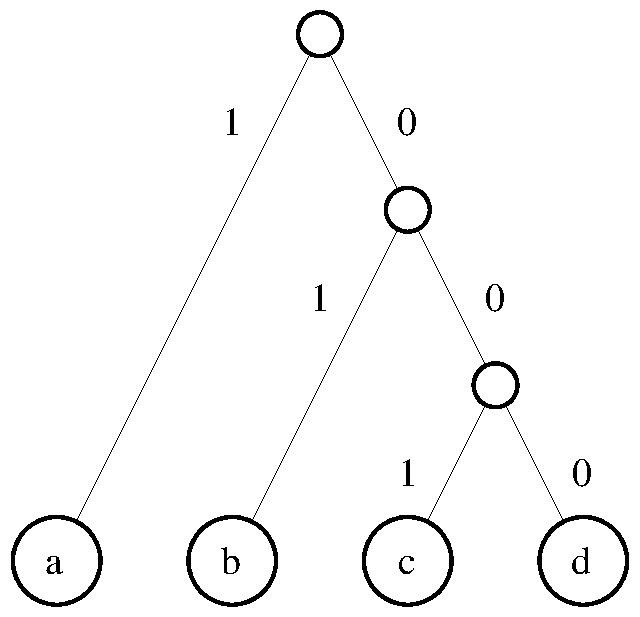
\includegraphics[scale=0.4]{images/Huffman}
		\end{center}
	}
\end{frame}
\subsection{Aufgabe B11 A3}
\begin{frame}
	\frametitle{Aufgabe B11 A3}
	Gegeben sei eine Quelle mit Alphabet $\{A,B,C,D\}$ und mit den folgenden
	Wahrscheinlichkeiten:\\
	$P(A)=\frac{1}{2}, P(B)=\frac{1}{4}, P(C)=\frac{1}{8}, P(D)=\frac{1}{8}$
	\begin{itemize}
	\only<1>{
		\item Berechnen Sie die Entropie der Quelle!
		\item Erstellen Sie eine entsprechende Huffman-Codierung!
		\item Was ist die mittlere Codewortl"ange? Gibt es einen Zusammenhang zur Entropie?
		}
		\only<2>{
		\item Gegeben sei der folgende Huffman-Baum:
		\begin{center}
			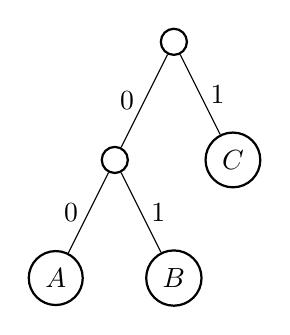
\begin{tikzpicture}
				\node[circle,draw]{}
				child{
				  node[circle,draw]{}
				  child{
				    node[circle,draw]{$A$}
				    edge from parent
				    node[left]{\textbf{$0$}}
				  }
				  child{
				    node[circle,draw]{$B$}
				    edge from parent
				    node[right]{\textbf{$1$}}
				  }
				  edge from parent
				  node[left]{\textbf{$0$}}
				}
				child{
				  node[circle,draw]{$C$}
				  edge from parent
				  node[right]{\textbf{$1$}}
				};
			\end{tikzpicture}
		\end{center}
		Dekodieren Sie $011011101100101011$! Ist der Huffman-Code geeignet?
		}
	\end{itemize}
\end{frame}

\section{Schluss}
\subsection{Schluss}
\begin{frame}
\frametitle{Bis zum nächsten Mal!}
%TODO change the comic
\begin{center}
	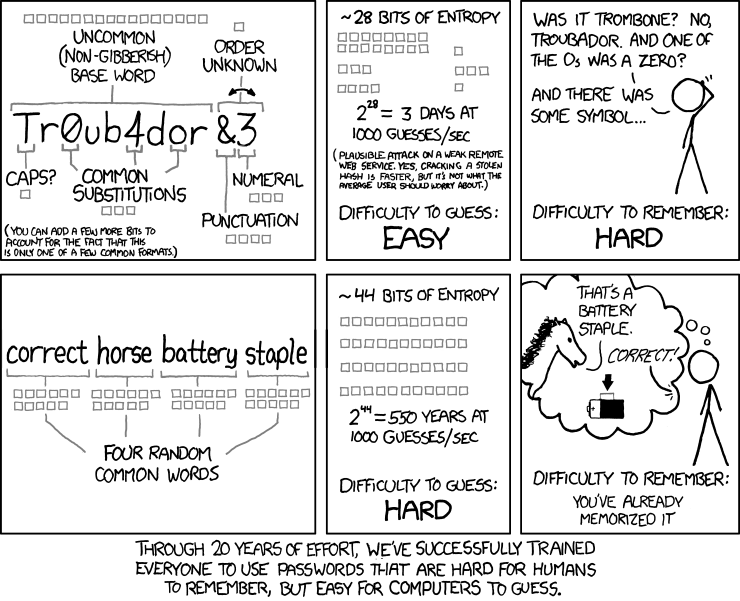
\includegraphics[height=0.85\textheight]{images/password_strength_936}
\end{center}
\end{frame}

\frame{
  \frametitle{Lizenzen}
  \center
  
\includegraphics[width=2em]{images/by}
  
\includegraphics[width=2em]{images/cc}
  
\includegraphics[width=2em]{images/sa}
  \\
  {\tiny

Dieses Werk ist unter einem ``Creative Commons Namensnennung-Weitergabe unter gleichen Bedingungen 3.0 Deutschland``-Lizenzvertrag lizenziert. Um eine Kopie der Lizenz zu erhalten, gehen Sie bitte zu \href{http://creativecommons.org/licenses/by-sa/3.0/de/}{http://creativecommons.org/licenses/by-sa/3.0/de/} oder schreiben Sie an Creative Commons, 171 Second Street, Suite 300, San Francisco, California 94105, USA.\\
  \vspace{1cm}
  Davon ausgenommen sind das Titelbild, welches aus der März-April 2002 Ausgabe von American Scientist erschienen ist und ohne Erlaubnis verwendet wird, sowie das KIT Beamer Theme. Hierfür gelten die Bestimmungen der jeweiligen Urheber.
  \vspace{1cm}
  \\ 
  }
  %Habe hier die Reihenfolge etwas umgestellt, weil die Formatierung bei mir komisch aussah. 
  %Wenn es bei dir anders ist, kannst du es auch wieder zurückändern, dann haben wir unterschiedliche Kompilieroptionen
}

\end{document}